% \textbf{Findings}
% \begin{enumerate}
%     \item Chat template significantly reduce repetition. It's not well-known/common practice by developers to use Chat template, in LLM application development. 
%     \item For generic prompt, increasing RPP normally reduce repetition. With Chat template model, the impact of \rpp is not as effective, for some model, increasing too high RPP can lead to higher repetition 
%     \item We show that RPP also have impact on the performance, so a balance approach can be achieved with RAP (with minimal findings)
% \end{enumerate}

% \textbf{Experiments}
% \begin{enumerate}
%     \item Impact of RPP on Repetition and Performance: showing results of all models, all datasets, all prompts. (@Donghao)
%     \item Optimizing the trade-off between performance and repetition. Objective is to show how to tune \rpp using RAP. (Existing content, maybe shorten). Remove numbers, change MTR to RR. Add for MT (@Donghao) 
%     \item comparing the best original + \rap of all models. The figures combining of figure-1-like figures. 
%     \item What is the percentages of responses having repetition, if having repetition, how severe it is? Choose few models and show the results. 
% \end{enumerate}



% \begin{align}
%     Gain = \frac{RR_{Origin} - RR_{RAP}}{P_{origin} - P_{RAP}}
% \end{align}

\subsection{Impact of \rpp on Repetition and Performance}
\label{subsec:impact_of_rpp}
\begin{figure*}[ht!]
    \centering
    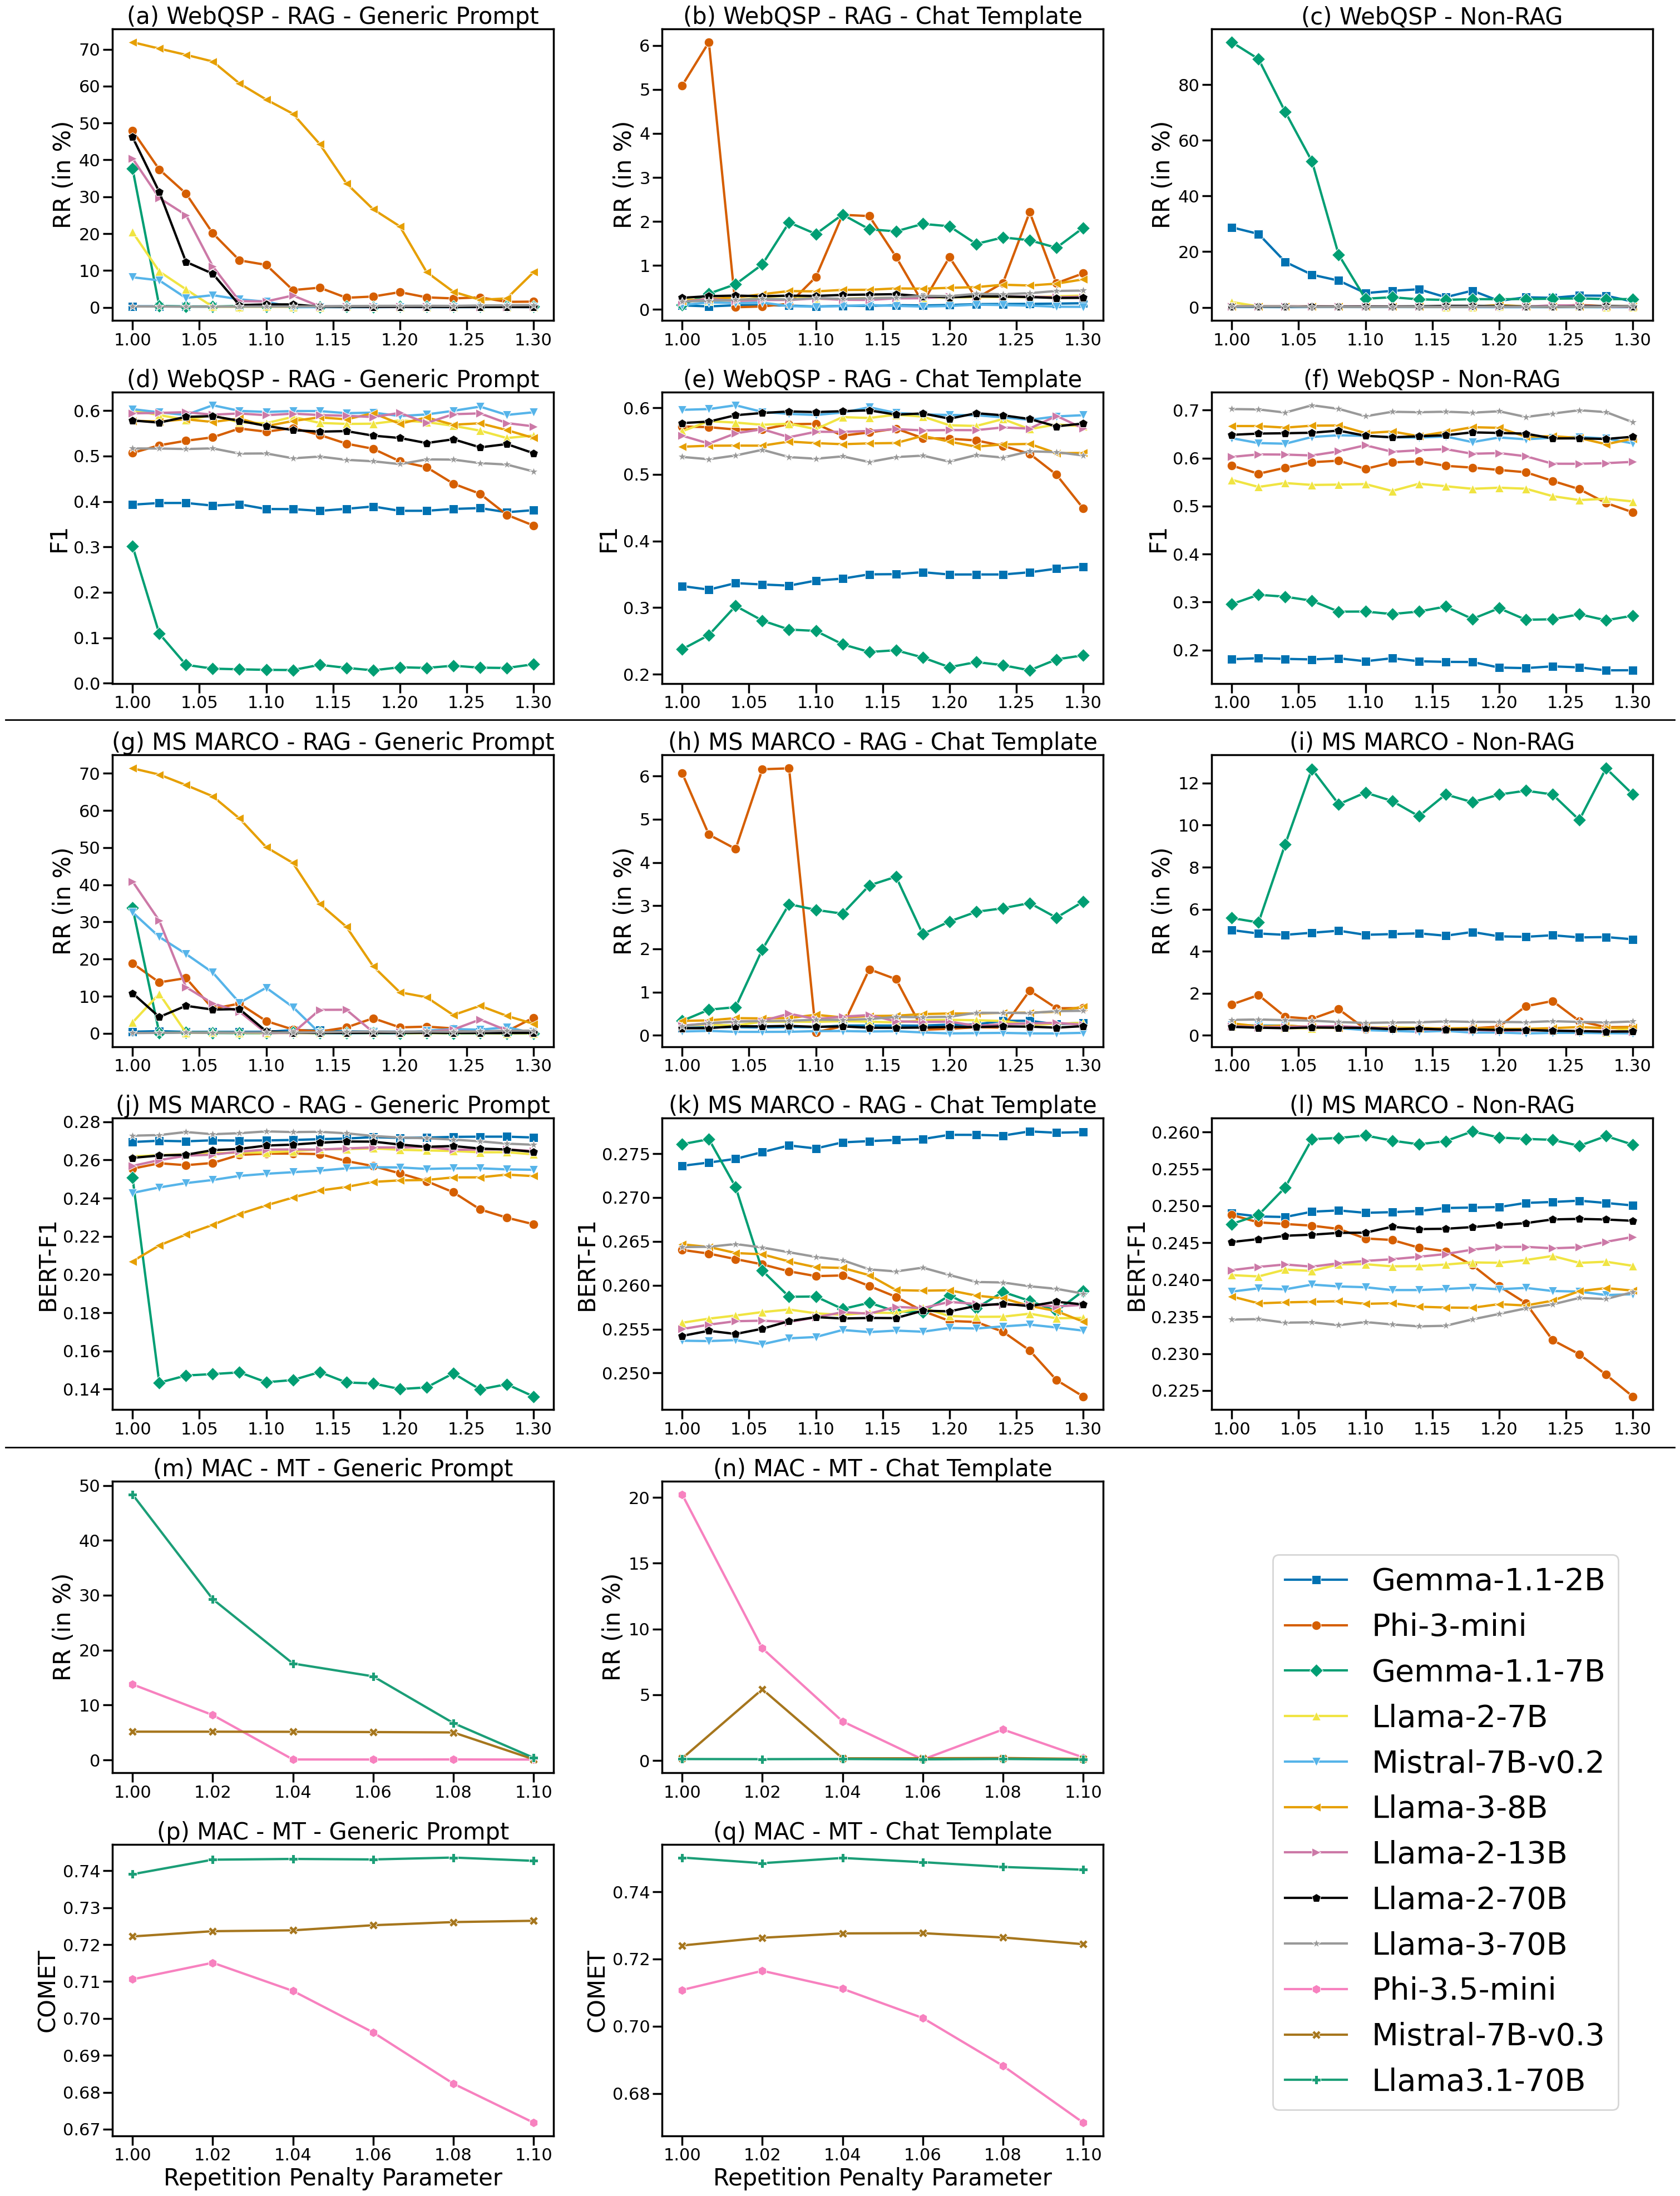
\includegraphics[width=\textwidth]{image/all-metrics-across-models_v2.png}
    \caption[Performance and Repetition Metrics Across Models]{
    Illustrating the impact of \rpp on \rr and performance across models, datasets, and prompting strategies. 
    % Results highlight the effectiveness of Chat Templates in reducing repetition while maintaining competitive performance, as well as the diminishing returns of increasing RPP beyond certain thresholds.
    % Performance and \rr when varying \rpp. This figure illustrates the impact of \rpp on repetition (RR) and performance (F1, BERT-F1, COMET) across different models, datasets (WebQSP, MS MARCO, MAC), and prompting strategies. Results highlight the effectiveness of Chat Templates in reducing repetition while maintaining competitive performance, as well as the diminishing returns of increasing RPP beyond certain thresholds.
    %\todo{to make subfigure title much bigger, can we draw a line between datasets?}
    }
    \label{fig:all-metrics-across-models_v2}
\end{figure*}

Figures \ref{fig:all-metrics-across-models_v2} illustrates the impact of \rpp on the repetition and performance of different open-source LLMs on the three datasets, using different prompting strategies. 
The results show that increasing RPP generally reduces repetition across strategies and datasets but often leads to a decline in performance. The trending and severity vary by model; for instance, while Phi-3-mini’s performance on MS MARCO-RAG-GP dropped significantly with RPP above 1.14, Llama-3-8B showed improved performance with higher RPP values under the same conditions. 
% The trade-off between reducing repetition and maintaining accuracy becomes evident beyond 1.15–1.20.
Therefore, selecting an optimal RPP value is crucial to balance repetition reduction with minimal impact on performance.
% metrics like F1, BERT-F1, or COMET.
%dataset

The datasets also show different behaviors. WebQSP generally exhibits higher repetition levels (e.g., at RPP = 1.0) than MS MARCO, especially with the RAG-GP strategy. This indicates that the nature of the dataset and task also influence repetition tendencies. In MAC dataset, despite a smaller RPP range tested, repetition still decreases as RPP increases. For both QA datasets, the Chat Template strategy consistently reduces repetition, showing lower RR values than the Generic Prompt approach. This suggests that the Chat Template effectively minimizes repetition in QA tasks. However, it surprisingly does not offer the same benefit for MT task, where increasing RPP effectively reduces repetition.



% Unlike QA tasks, the Chat Template and Generic Prompt strategies show similar repetition levels in MT.

% Chat template 
% Impact of RPP 
% , but Llama-3-8B in the same setting gets higher performance with higher value of RPP. 

% Several key insights can be drawn from these results:

% \noindent 
% \textbf{Chat Template Superiority}: 
% Across both QA datasets and all RPP values, the Chat Template strategy consistently achieves the lowest levels of repetition. This is reflected in lower RR values compared to the Generic Prompt approach. These results suggest that using a Chat Template is an effective method for minimizing repetitive content in model outputs for QA task. Supperisingly, using template does not seem to help for machine translation, although repetition can be reduced easily by increasing \rpp for this task. 

% \noindent 
% \textbf{The impact of RPP}: the results show that increasing RPP generally reduces repetition across different strategies and datasets. 
% However, it is also shown that using higher RPP value often leads to a decline in performance for most of the models and settings. The severity of the impact varies depending on the model. For example, Phi-3-mini's performance in MS MARCO-RAG-Generic Prompt significantly reduced when using RPP higher than 1.14.
% The impact is particularly noticeable as RPP increases beyond 1.15--1.20, where the trade-off between reducing repetition and maintaining model accuracy becomes evident. Therefore, it is important to choose an optimal RPP value that balances the reduction in repetition with minimal impact on performance (F1, BERT-F1, or COMET).
% \noindent \textbf{Diminishing Returns}: For most strategies, the reduction in repetition plateaus as RPP increases beyond certain thresholds (typically around 1.20--1.25). This indicates that there may be an optimal range for RPP settings, beyond which further increases provide minimal additional benefits in terms of repetition reduction. 

% \noindent \textbf{Dataset Differences}: The behaviors are also different in the different datasets. WebQSP dataset generally exhibits higher baseline repetition levels (at RPP = 1.0) compared to MS MARCO, particularly for the RAG - Generic Prompt strategy. This indicates that the nature of the dataset and task can significantly influence repetition tendencies. In the MAC machine translation (MT) task, although a smaller range of RPP values was tested, repetition reduction is still evident as RPP increases. Interestingly, unlike the QA tasks, the Chat Template and Generic Prompt strategies show comparable levels of repetition in the MT task.

% These findings highlight the importance of carefully tuning the RPP and selecting appropriate prompting strategies to optimize model performance while minimizing undesirable repetition. The results also underscore the effectiveness of Chat Templates in managing repetition across different models and datasets.

% Figure \ref{fig:mean-metrics-across-models} shows the results of average mean total repetitions and performance when varying \rp.  


% \textbf{Mean Total Repetitions:} Increasing RPP generally reduces mean total repetitions across all models and prompt templates, indicating that a higher RPP effectively suppresses repetitive content. The \raggen exhibits the highest repetition issues, with mean total repetitions exceeding 600 at an RPP of 1.0, gradually decreasing as RPP increases. Repetition issues generally cease when RPP is greater than or equal to 1.2, a trend consistent across other prompt templates.

% \textbf{Performance Metrics}: For the WebQSP dataset (Figures \ref{fig:mean-metrics-across-models}a and \ref{fig:mean-metrics-across-models}c), increasing RPP stabilizes or slightly reduces F1 scores for \raggen and \ragtem, while Non-RAG methods maintain relatively stable F1 scores. For the MS MARCO dataset (Figures \ref{fig:mean-metrics-across-models}b and \ref{fig:mean-metrics-across-models}d), overall performance declines with increasing RPP for \raggen and \ragtem, while Non-RAG methods remain stable.




% \textbf{Mean Total Repetitions:} Increasing RPP generally reduces mean total repetitions across all models and prompt templates, indicating that a higher RPP effectively suppresses repetitive content. The \raggen exhibits the highest repetition issues, with mean total repetitions exceeding 600 at an RPP of 1.0, gradually decreasing as RPP increases. Repetition issues generally cease when RPP is greater than or equal to 1.2, a trend consistent across other prompt templates.

% \textbf{Performance Metrics:} For the WebQSP dataset (Figures \ref{fig:mean-metrics-across-models}a and \ref{fig:mean-metrics-across-models}c), increasing RPP tends to stabilize or slightly reduce F1 scores for \raggen and \ragtem. Non-RAG methods maintain relatively stable F1 scores across different RPP values. Conversely, for the MS MARCO dataset (Figures \ref{fig:mean-metrics-across-models}b and \ref{fig:mean-metrics-across-models}d), overall performance gradually declines with increasing RPP for \raggen and \ragtem, while Non-RAG methods exhibit greater stability.




% Interestingly, for WebQSP, Non-RAG methods provide the highest F1 scores across all RPP values, whereas for MS MARCO, they yield the lowest overall performance scores. This discrepancy likely arises from using BLEU-1 and ROUGE-L metrics for MS MARCO, which have lower correlation with human ratings \cite{clinciu2021study}, penalizing human-like LLM responses. Future work will explore embedding-based evaluation methods, like BERTScore and BLEURT, which correlate better with human ratings.
% While general trends in Figure \ref{fig:mean-metrics-across-models} are consistent across most models, several notable exceptions are identified. 
% Phi-3-mini Model with \ragtem (WebQSP and MS MARCO): Beyond an RPP of 1.24, total repetitions increase significantly (Figures \ref{fig:webqsp-metrics}b and \ref{fig:ms-marco-metrics}b), deviating from the expected trend. This model shows a sudden increase in answer length and text abnormalities beyond an RPP of 1.24.
% Phi-3-mini Model with Non-RAG Template (MS MARCO): Increasing RPP beyond 1.2 results in a sharp rise in total repetitions (Figure \ref{fig:ms-marco-metrics}c), indicating sensitivity to higher RPP values. This model also shows increased answer length and text abnormalities.
% Gemma-1.1-7b Model with Non-RAG Template (MS MARCO): Total repetitions increase significantly beyond an RPP of 1.04 and do not decrease with further RPP increases (Figure \ref{fig:ms-marco-metrics}c), suggesting ineffective repetition suppression. This model shows increased newline and space repetitions beyond an RPP of 1.04, as it tries to format answers in bullet points. Additional details are in Appendix \ref{app:impact_of_rpp}.
% The impact of RPP on repetition and performance varies across models and prompting strategies. While increasing RPP generally reduces repetitions, it can also negatively affect performance metrics like F1 scores. RAG methods, especially using the Generic Prompt, exhibit significant fluctuations, necessitating careful tuning to balance repetition suppression with maintaining high performance quality.






% % Please add the following required packages to your document preamble:
% \usepackage{multirow}
\begin{table*}[t]
\centering
\resizebox{.85\textwidth}{!}{
\begin{tabular}{l|l|rrrr|rrrr|rrrr}
\toprule
\multirow{2}{*}{Dataset}   & \multirow{2}{*}{Model} & \multicolumn{4}{c|}{RAG - Generic Prompt}                                                                & \multicolumn{4}{c|}{RAG - Chat Template}                                                                 & \multicolumn{4}{c}{Non-RAG}                                                                             \\ \cline{3-14} 
                           &                        & \multicolumn{1}{c}{RPP} & \multicolumn{1}{c}{MTR} & \multicolumn{1}{c}{Perf.} & \multicolumn{1}{c|}{RAP} & \multicolumn{1}{c}{RPP} & \multicolumn{1}{c}{MTR} & \multicolumn{1}{c}{Perf.} & \multicolumn{1}{c|}{RAP} & \multicolumn{1}{c}{RPP} & \multicolumn{1}{c}{MTR} & \multicolumn{1}{c}{Perf.} & \multicolumn{1}{c}{RAP} \\ \hline
\multirow{18}{*}{WebQSP}   & Gemma-1.1-2B       & 1.04                    & 0.00                    & 39.7                    & 39.7                   & 1.30                    & 0.01                    & 36.1                    & 36.1                   & 1.20                    & 0.08                    & 16.3                    & 16.3                  \\\cmidrule{2-14}
                           % & Gemma-1.1-2B-F1           & 1.04                    & 0.00                    & 39.7                    & 39.7                   & 1.30                    & 0.01                    & 36.1                    & 36.1                   & 1.02                    & 51.67                   & 18.3                    & 10.2                  \\ \cmidrule{2-14}
                           & Gemma-1.1-7B       & 1.00                    & 35.46                   & 30.2                    & 18.2                   & 1.04                    & 0.09                    & 30.2                    & 30.1                   & 1.16                    & \textcolor{blue}{1.21}                    & 29.1                    & 27.7                  \\
                           & Gemma-1.1-7B-F1           & 1.00                    & 35.46                   & 30.2                    & 18.2                   & 1.04                    & 0.09                    & 30.2                    & 30.1                   & 1.02                    & \textcolor{blue}{633.61}                  & 31.5                    & 11.2                  \\\cmidrule{2-14}
                           & Llama-2-7B         & 1.06                    & \textcolor{blue}{0.01}                    & 58.9                    & 58.9                   & 1.16                    & 0.02                    & 59.0                    & 58.9                   & 1.00                    & 0.02                    & 54.8                    & 54.8                  \\
                           & Llama-2-7B-F1             & 1.00                    & \textcolor{blue}{78.48}                   & 60.1                    & 30.9                   & 1.16                    & 0.02                    & 59.0                    & 58.9                   & 1.00                    & 9.09                    & 55.5                    & 43.3                  \\\cmidrule{2-14}
                           & Llama-2-13B        & 1.20                    & 0.00                    & 59.5                    & 59.5                   & 1.28                    & 0.00                    & 58.8                    & 58.8                   & 1.10                    & 0.29                    & 62.7                    & 61.9                  \\
                           % & Llama-2-13B-F1            & 1.04                    & 62.02                   & 59.6                    & 32.1                   & 1.28                    & 0.00                    & 58.8                    & 58.8                   & 1.10                    & 0.29                    & 62.7                    & 61.9                  \\\cmidrule{2-14}
                           & Llama-2-70B        & 1.16                    & 0.00                    & 55.5                    & 55.5                   & 1.14                    & 0.03                    & 59.6                    & 59.5                   & 1.08                    & 0.19                    & 65.7                    & 65.2                  \\ \cmidrule{2-14}
                           % & Llama-2-70B-F1            & 1.06                    & 21.57                   & 58.8                    & 39.2                   & 1.14                    & 0.03                    & 59.6                    & 59.5                   & 1.08                    & 0.19                    & 65.7                    & 65.2                  \\\cmidrule{2-14}
                           & Llama-3-8B         & 1.26                    & \textcolor{blue}{9.96}                    & 57.2                    & 44.0                   & 1.18                    & 0.01                    & 55.8                    & 55.8                   & 1.06                    & 0.02                    & 66.8                    & 66.7                  \\
                           & Llama-3-8B-F1             & 1.18                    & \textcolor{blue}{178.99}                  & 59.4                    & 26.1                   & 1.18                    & 0.01                    & 55.8                    & 55.8                   & 1.08                    & 0.07                    & 66.8                    & 66.6                  \\\cmidrule{2-14}
                           & Llama-3-70B        & 1.06                    & 0.00                    & 51.7                    & 51.7                   & 1.06                    & 0.00                    & 53.7                    & 53.7                   & 1.06                    & 0.02                    & 71.0                    & 70.9                  \\
                           % & Llama-3-70B-F1            & 1.06                    & 0.00                    & 51.7                    & 51.7                   & 1.06                    & 0.00                    & 53.7                    & 53.7                   & 1.06                    & 0.02                    & 71.0                    & 70.9                  \\\cmidrule{2-14}
                           & Mistral-7B         & 1.26                    & 0.01                    & 60.9                    & 60.8                   & 1.04                    & 0.00                    & 60.4                    & 60.4                   & 1.08                    & 0.00                    & 64.8                    & 64.8                  \\
                           % & Mistral-7B-F1             & 1.06                    & 14.74                   & 61.2                    & 43.9                   & 1.04                    & 0.00                    & 60.4                    & 60.4                   & 1.08                    & 0.00                    & 64.8                    & 64.8                  \\\cmidrule{2-14}
                           & Phi-3-mini         & 1.16                    & 15.42                   & 52.7                    & 37.5                   & 1.08                    & 0.02                    & 57.5                    & 57.5                   & 1.08                    & 0.07                    & 59.5                    & 59.3                  \\
                           % & Phi-3-mini-F1             & 1.12                    & 34.94                   & 56.2                    & 34.0                   & 1.10                    & 1.23                    & 57.6                    & 54.8                   & 1.08                    & 0.07                    & 59.5                    & 59.3                  \\ 
                           \midrule
% \multirow{18}{*}{MS MARCO} & Gemma-1.1-2b
\multirow{9}{*}{\begin{tabular}[c]{@{}l@{}}MS \\ MARCO\end{tabular}} & Gemma-1.1-2b       & 1.00                    & 0.87                    & 32.6                    & 31.5                   & 1.02                    & 0.00                    & 34.6                    & 34.6                   & 1.16                    & 1.28                    & 10.0                    & 9.5                   \\
                           % & Gemma-1.1-2b           & 1.00                    & 0.87                    & 32.6                    & 31.5                   & 1.02                    & 0.00                    & 34.6                    & 34.6                   & 1.16                    & 1.28                    & 9.96                    & 9.47                  \\
                           & Gemma-1.1-7B       & 1.00                    & 29.76                   & 18.5                    & 11.6                   & 1.00                    & 0.00                    & 29.9                    & 29.9                   & 1.02                    & 1.884                   & 9.9                     & 9.2                   \\
                           % & Gemma-1.1-7b           & 1.00                    & 29.76                   & 18.5                    & 11.6                   & 1.00                    & 0.00                    & 29.9                    & 29.9                   & 1.02                    & 1.88                    & 9.93                    & 9.24                  \\
                           & Llama-2-7B        & 1.06                    & 0.13                    & 25.2                    & 25.1                   & 1.00                    & 0.15                    & 16.8                    & 16.7                   & 1.04                    & 0.09                    & 9.6                     & 9.6                   \\
                           % & Llama-2-7b             & 1.06                    & 0.13                    & 25.2                    & 25.1                   & 1.00                    & 0.15                    & 16.8                    & 16.7                   & 1.04                    & 0.09                    & 9.62                    & 9.59                  \\
                           & Llama-2-13B        & 1.10                    & 0.00                    & 27.5                    & 27.5                   & 1.00                    & 0.02                    & 17.1                    & 17.0                   & 1.02                    & 0.95                    & 10.3                    & 9.9                   \\
                           % & Llama-2-13b            & 1.10                    & 0.00                    & 27.5                    & 27.5                   & 1.10                    & 0.04                    & 17.1                    & 17.0                   & 1.02                    & 0.95                    & 10.29                   & 9.90                  \\
                           & Llama-2-70B        & 1.12                    & 0.00                    & 24.0                    & 24.0                   & 1.10                    & 0.00                    & 17.9                    & 17.9                   & 1.18                    & 0.03                    & 9.3                     & 9.3                   \\
                           % & Llama-2-70b            & 1.12                    & 0.00                    & 24.0                    & 24.0                   & 1.10                    & 0.00                    & 17.9                    & 17.9                   & 1.04                    & 0.02                    & 9.27                    & 9.27                  \\
                           & Llama-3-8B         & 1.24                    & 42.49                   & 8.7                     & 5.0                    & 1.00                    & 0.02                    & 24.4                    & 24.4                   & 1.10                    & 0.16                    & 9.7                     & 9.6                   \\
                           % & Llama-3-8B             & 1.20                    & 132.98                  & 9.9                     & 4.6                    & 1.00                    & 0.02                    & 24.4                    & 24.4                   & 1.12                    & 0.20                    & 9.70                    & 9.62                  \\
                           & Llama-3-70B        & 1.00                    & 0.00                    & 33.7                    & 33.7                   & 1.00                    & 0.02                    & 24.9                    & 24.8                   & 1.04                    & 0.04                    & 9.3                     & 9.3                   \\
                           % & Llama-3-70B            & 1.00                    & 0.00                    & 33.7                    & 33.7                   & 1.00                    & 0.02                    & 24.9                    & 24.8                   & 1.04                    & 0.04                    & 9.29                    & 9.27                  \\
                           & Mistral-7B         & 1.20                    & 0.00                    & 22.3                    & 22.3                   & 1.12                    & 0.00                    & 23.6                    & 23.6                   & 1.00                    & 0.23                    & 10.8                    & 10.7                  \\
                           % & Mistral-7B             & 1.20                    & 0.00                    & 22.3                    & 22.3                   & 1.12                    & 0.00                    & 23.6                    & 23.6                   & 1.02                    & 0.38                    & 10.81                   & 10.63                 \\
                           & Phi-3-mini         & 1.14                    & 0.46                    & 15.5                    & 15.2                   & 1.10                    & 0.06                    & 27.3                    & 27.3                   & 1.10                    & 0.34                    & 10.7                    & 10.6                  \\ \bottomrule
                           % & Phi-3-mini             & 1.14                    & 0.46                    & 15.5                    & 15.2                   & 1.02                    & 10.20                   & 31.2                    & 23.9                   & 1.00                    & 8.01                    & 11.99                   & 9.55                 
\end{tabular}}
\caption{Performance comparison between open-source LLMs for two datasets \webqsp and \ms. 
For each model, we choose the repetition penalty parameter (\rp) based on the best repetition-aware performance (\rap), the mean total repetition (\mtr), and the original F1 scores (Perf.). We also report the best results tuned based on the original F1 scores for \webqsp ([MODEL-NAME]-F1). Drastic changes in terms of repetition are highlighted in blue text. Results tuned using the original F1 is denoted in format [MODEL-NAME]-F1.}
%Performance comparison between open-source LLMs for two datasets \webqsp and \ms. For each model, we choose the repetition penalty parameter (\rp) based on the best repetition-aware performance (\rap). We also report the corresponding mean total repetition (\mtr) for each model. Results of different prompting strategies including RAG - Generic Prompt, RAG - Chat Template, and Non-RAG are reported. The performance (Perf.) is the original F1 scores for \webqsp or \hm for \ms. To demonstrate the beneficial of our framework, we also report the best results tuned based on the original F1 scores for \webqsp ([MODEL-NAME]-F1). Drastic changes in terms of repetition are highlighted in blue text. 
\label{tab:best_rpp}
\end{table*}

\input{tab_best_rap}

\subsection{Optimizing the Trade-Off Between Performance and Repetition}
\label{sec:eval_tuning}

% Figure \ref{fig:performance_vs_repetition} illustrates the balance between performance and reducing excessive repetition for the Phi-3-mini model across various datasets and prompt types. The blue lines represent the original performance scores (F1 or overall performance), the orange lines (scaled on the right y-axis) denote the mean total repetitions (MTR) across the dataset, and the green lines indicate the repetition-aware performance (RAP). Each subplot displays results and different dataset and prompt type configurations, with the blue vertical bar centered around the Repetition Penalty Parameter (RPP) that yields the best original performance, and the orange bar positioned at the RPP with the best RAP. The separation or overlap of these bars indicates the trade-off between performance and repetition for different RPP values.

% Observations from these configurations indicate that higher RPP values generally lead to a reduction in MTR across most datasets and prompt types. For instance, in WebQSP with \raggen (subplot a), the original performance remains high up to an RPP value of around 1.15, beyond which it starts to decline, while the MTR significantly decreases. Conversely, in the MS MARCO dataset with Non-RAG (subplot f), the overall performance remains relatively stable across a range of RPP values, but there is a clear optimal point where the best RAP is achieved. This suggests that while increasing the RPP can effectively reduce repetition, it is crucial to strike a balance to maintain high performance. The overlap of blue and orange bars in subplots (c) and (d) indicates configurations where the optimal RPP for both original performance and RAP coincide, highlighting the potential for achieving both goals simultaneously in certain setups.

% The relationship between MTR and RPP is evident across all configurations. As the RPP increases, the MTR consistently decreases, indicating that a higher repetition penalty effectively suppresses repetitive content. However, it is also observed that when the RPP exceeds certain values, the MTR begins to increase again. This trend is most prominent in RAG configurations, where the initial levels of MTR are considerably higher. For instance, in subplot (b), the MTR starts at a high value and declines as the RPP increases, reaching its minimum at an RPP value of 1.15, but then starts to rise again when the RPP is set too high. This demonstrates the efficacy of RPP in controlling repetition, but also underscores the importance of selecting the optimal RPP to avoid negatively impacting overall performance. The balance achieved through RAP highlights the need for an optimal RPP that minimizes repetitions without compromising response quality.

% Comparing performance across different prompt types, it is evident that \ragtem generally results in better performance metrics than \raggen and Non-RAG methods. For example, in subplots (b) and (e), the performance scores remain higher for a broader range of RPP values compared to their Generic Prompt counterparts. Non-RAG configurations, while less prone to repetitions, often exhibit lower performance metrics in tasks requiring complex retrieval-based responses, as seen in the MS MARCO dataset. Therefore, we recommend utilizing the \ragtem for tasks where high-quality, non-repetitive responses are critical, and carefully adjusting the RPP to optimize both performance and repetition suppression.

% \todo{@Donghao: To first explain this experiment. That we compare the best performance when tuning using the original metric vs. using RAP. That what we want to compare here. E.g., the reduction of Performance vs. the reduction of RR? It seems like we are describing the figures, but not providing any insights here. What we learn from these results? }
\begin{figure*}[ht!]
    \centering
    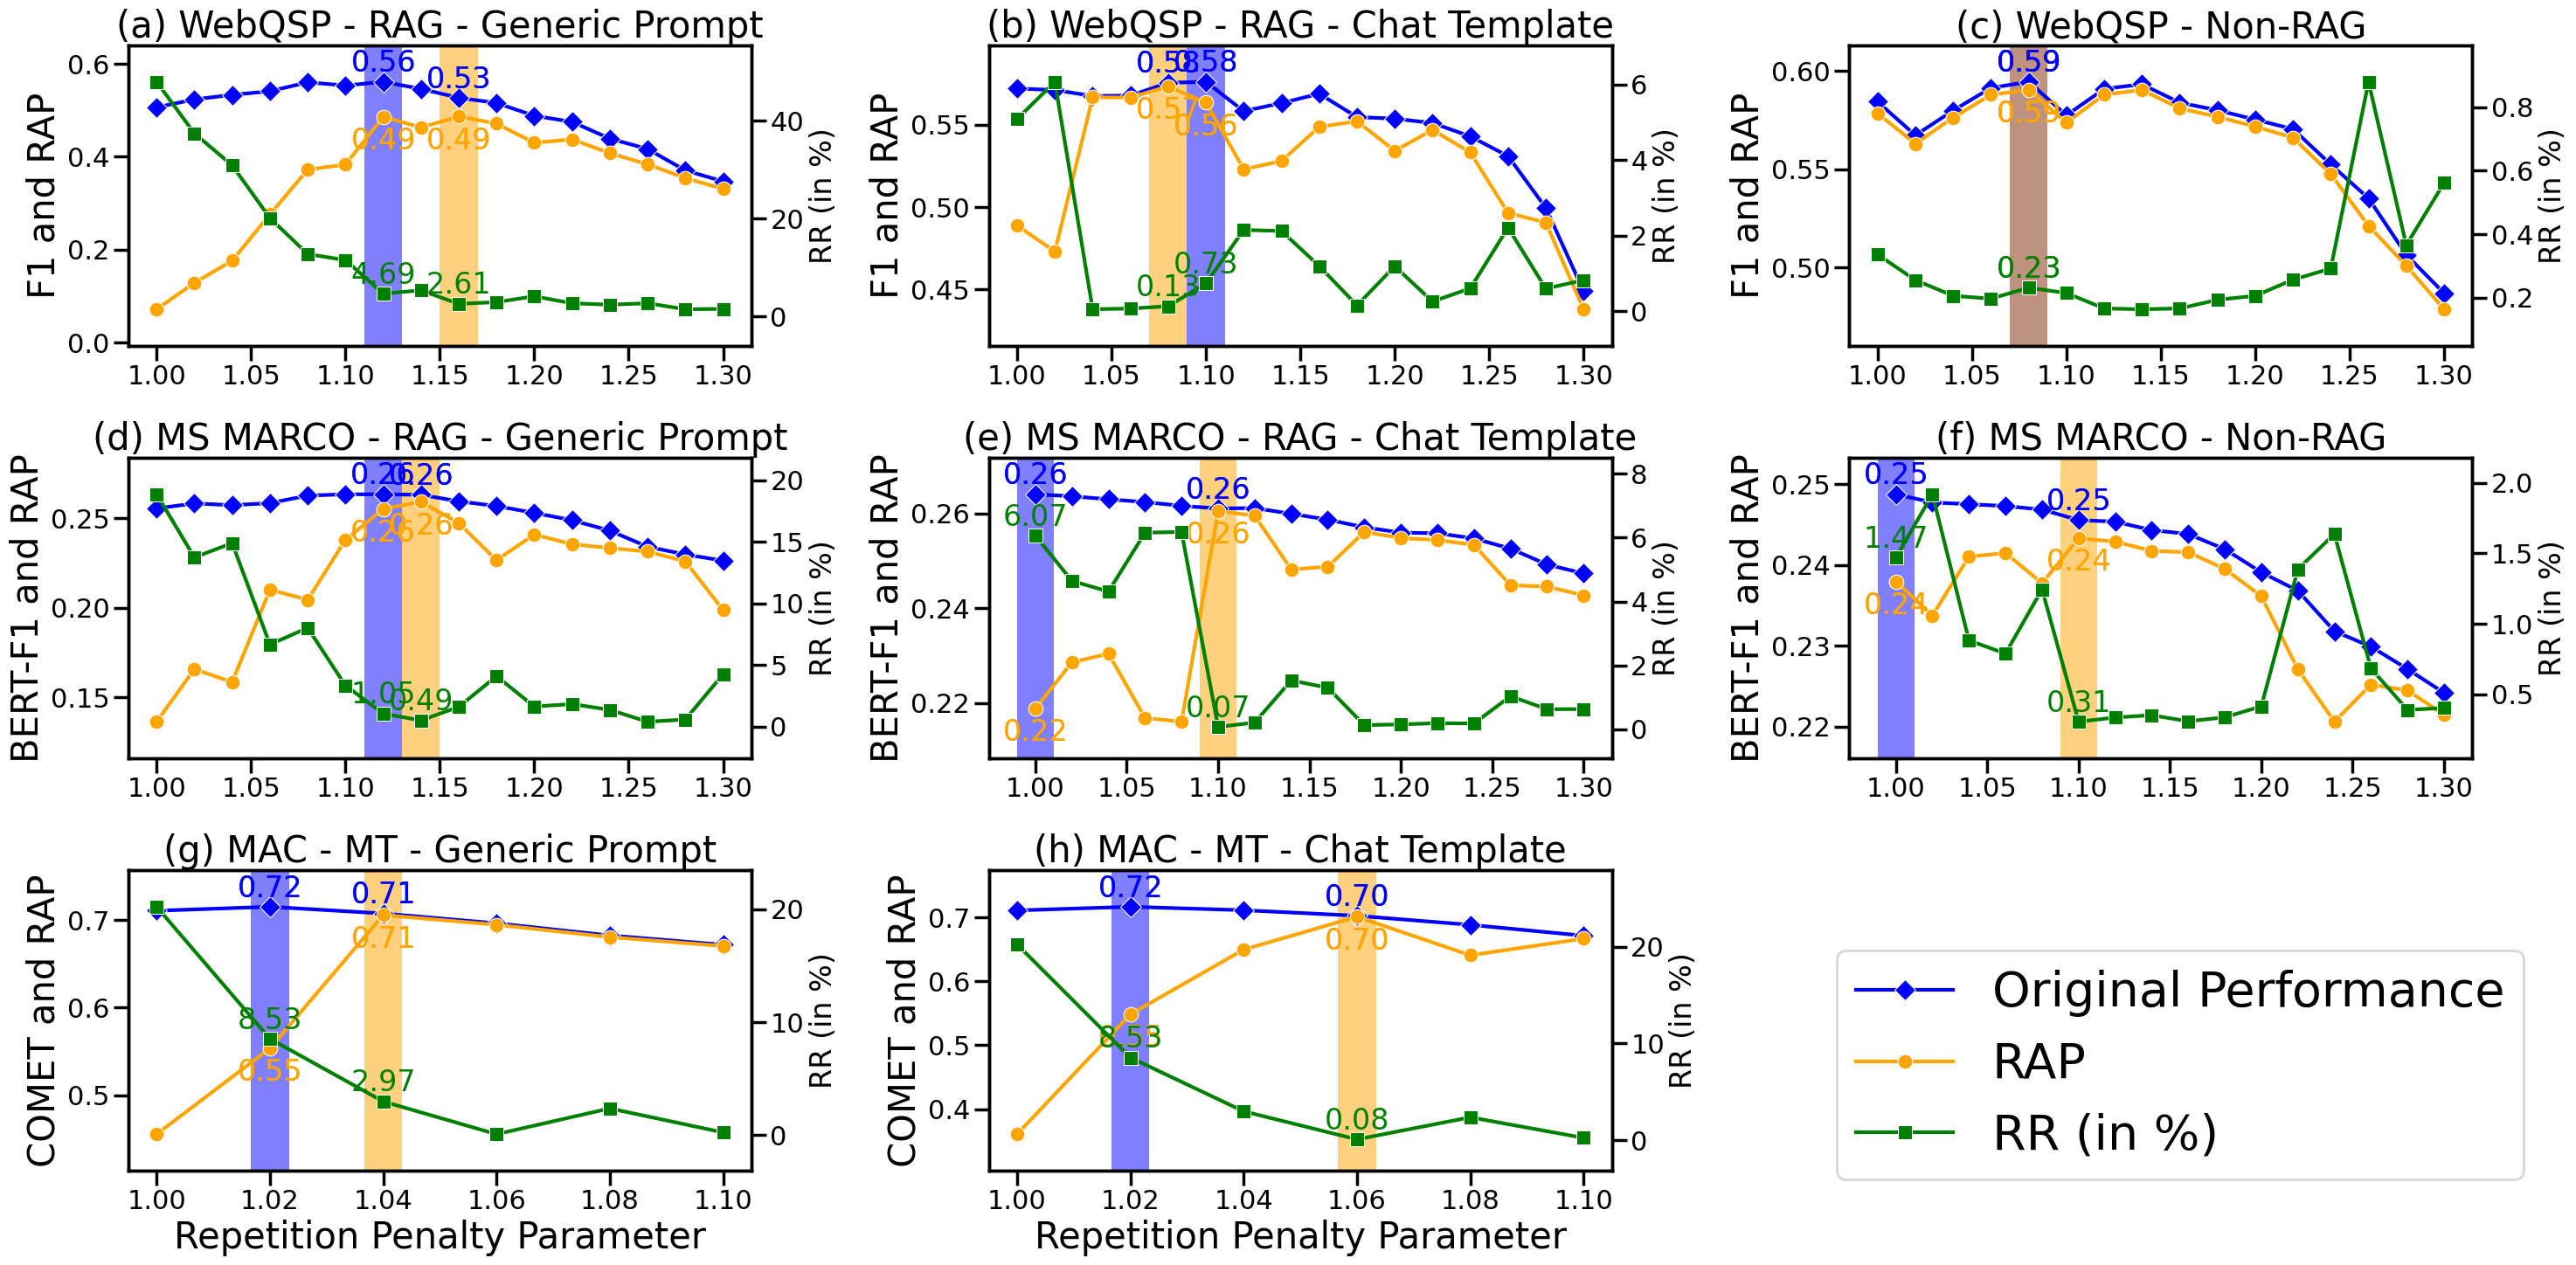
\includegraphics[width=1\textwidth]{image/performance_vs_repetition_v2.png}
    \caption[Performance vs. Repetition Trade-Off]{
    Illustrating original performance, repetition-aware performance (RAP), and repetition ratio (RR) while varying \rpp. Results are shown for Phi-3-mini in QA (Subplots (a) to (f)) and Phi-3.5-mini  in machine translation (Subplots (g) and (h)).
    % Illustrating the original performance, repetition-aware performance (RAP), and repetition ratio (RR) when varying \rpp. Results are shown for the Phi-3-mini model in QA (Subplots (a) to (f)) and the Phi-3.5-mini model in machine translation (Subplots (g) and (h)). 
    % The blue line indicates original performance (F1, BERT-F1, or COMET), the orange line represents RAP, and the green line shows RR in percentage. 
    The blue shaded region highlights the RPP for optimal original performance, while the orange region indicates the RPP for the best RAP; overlapping regions are marked in brown to show alignment.
    % Performance vs. Repetition Trade-Off. This figure shows the original performance and repetition-aware performance (RAP), and the repetition ratio (RR) when varying \rpp, across different datasets and prompt types. We showcase results from Phi-3-mini model for question answering (a-f) and Phi-3.5-mini model for machine translation (g-h) tasks. 
    % The blue line represents the original performance (F1, BERT-F1, or COMET), the orange line represents RAP, and the green line shows \rr in percentage. 
    % The blue shaded region highlights the Repetition Penalty Parameter (RPP) for the best original performance, while the orange region highlights the RPP for the best RAP. When both regions overlap, the shaded area changes to brown to indicate this alignment. 
    % Performance vs. Repetition Trade-Off. This figure shows the balance between performance and repetition reduction across different datasets and prompt types. 
    % Subplots (a-c) present results for the Phi-3-mini model on the WebQSP dataset, and subplots (d-f) show results on the MS MARCO dataset, both with different prompting strategies. Subplots (g-h) illustrate results for the Phi-3.5-mini model on the MAC machine translation task, using various prompting strategies.
    % The blue line represents the original performance (F1, BERT-F1, or COMET), the orange line represents the Repetition-Aware Performance (RAP), and the green line shows the Repetition Ratio (RR) in percentage. 
    % The blue shaded region highlights the Repetition Penalty Parameter (RPP) for the best original performance, while the orange region highlights the RPP for the best RAP. When both regions overlap, the shaded area changes to brown to indicate this alignment. 
    }
    \label{fig:performance_vs_repetition_v2}
\end{figure*}
% We conducted experiments on various datasets and models, comparing performance using both original metrics (such as F1, BLEU, and COMET) and RAP.
% }
% When tuning using conventional metrics, the objective is purely to select the value of \rpp with best performance, but that might come with serious repetition problem. Whereas, 
% Our objective is to identify the optimal \rpp that maximizes RAP by balancing model performance with the reduction of repetition in the generated content.
%
% In this section, we demonstrate the use of \rap in tuning \rpp by comparing model performance and repetition issues when tuning RPP using conventional evaluation metrics versus \rap. 
% Figure \ref{fig:performance_vs_repetition_v2} illustrates the relationship between \rpp, model performance, and repetition across different datasets and prompt strategies. We showcase results of Phi-3-mini for WebQSP and \ms, and Phi-3.5-mini for MAC. 
% The blue lines represent the original performance scores (F1 for WebQSP, BERT-F1 for MS MARCO, and COMET for MAC), the orange lines show the \rap scores, and the green lines (scaled on the right y-axis) indicate \rr in percentage. 
% The blue shaded region highlights the \rpp for the best original performance, while the orange region highlights the RPP for the best RAP. When both regions overlap, the shaded area changes to brown to indicate this alignment. 

This section demonstrates the use of RAP in tuning RPP by comparing model performance and repetition when using conventional metrics (Original Performance) versus RAP. Figure \ref{fig:performance_vs_repetition_v2} shows the relationship between RPP, performance, and repetition for Phi-3-mini on WebQSP and MS MARCO, and Phi-3.5-mini on MAC. Blue lines represent original performance (F1 for WebQSP, BERT-F1 for MS MARCO, and COMET for MAC), orange lines show RAP scores, and green lines (right y-axis) indicate RR percentages. The blue shaded area marks the RPP with the best performance based on conventional metrics, the orange marks the best RAP, and brown indicates overlap between the two.

% In most of the shown cases (except for Figure \ref{fig:performance_vs_repetition_v2}c) the best values of \rpp when tuning using original performance are different from that when tuning using \rap. For example, in Figure \ref{fig:performance_vs_repetition_v2}e, when tuning using BERT-F1, the best \rpp is 1.0 where the performance is \todo{xx}, but the repetition ratio is very high at \todo{xx\%}. Whereas, using \rap, the best \rpp is 1.1, where the performance is \todo{xx} (drop \todo{xx\%}) but the repetition ratio drop significantly to \todo{xx\%} (drop \todo{xx\%)}. This shows that tuning \rpp using \rap helps find \rpp value that minimally reduce performance while significantly lowering repetition ratio. Another example with different visualization is illustrated in Figure \ref{fig:hook}. 

In most cases (except Figure \ref{fig:performance_vs_repetition_v2}c), the optimal RPP differs when tuning for original performance versus RAP. For instance, in Figure \ref{fig:performance_vs_repetition_v2}e, tuning with BERT-F1 gives the best RPP at 1.0 with a performance of 0.264, but the repetition ratio is high at 6.07\%. With RAP, the best RPP shifts to 1.1, where performance drops by 1.1\% (drop 0.003), but the repetition ratio significantly decreases by 98.8\% (drop 6\%). This demonstrates that tuning RPP with RAP helps balance performance with reduced repetition. Another example with different visualization is illustrated in Figure \ref{fig:hook}. 
These results highlight the importance of tuning RPP to balance performance and repetition reduction, which can be achieved using RAP. The optimal RPP varies by task, dataset, and prompting strategy. 

% These results underscore the importance of carefully tuning the RPP to achieve an optimal balance between model performance and repetition reduction, that can be achieved by tuning RPP based on \rap. The optimal RPP value varies depending on the task, dataset, and prompting strategy used.

% \noindent \textbf{WebQSP}: For WebQSP with RAG-Generic Prompt (subplot a), performance remains high up to an RPP of approximately 1.12 before declining, while RR decreases significantly. In contrast, the RAG-Chat Template (subplot b) shows more stable performance across a wider range of RPP values, with lower overall repetition.

% \noindent \textbf{MS MARCO}: The results for MS MARCO (subplots d-f) follow similar trends. RAG-Generic Prompt exhibits a more pronounced trade-off between performance and repetition compared to RAG-Chat Template and Non-RAG approaches.

% \noindent \textbf{MAC}: In the MAC machine translation task (subplots g-h), increasing the RPP beyond certain thresholds (around 1.02–1.04) leads to noticeable declines in performance, while effectively reducing repetition. Both Generic Prompt and Chat Template strategies show similar trends, with higher RPP reducing repetition but negatively impacting COMET scores beyond 1.04.

% Across all datasets and strategies, there is a clear trend of decreasing RR as RPP increases. However, an excessively high RPP can lead to performance degradation. The optimal RPP, typically marked by the peak of the RAP curve (orange line) and highlighted by the orange region in the subplots, often strikes a balance between maintaining high performance and minimizing repetition.

% These results underscore the importance of carefully tuning the RPP to achieve an optimal balance between model performance and repetition reduction, which can be achieved by finding the RPP that maximizes RAP. The optimal RPP value varies depending on the task, dataset, and prompting strategy used.

% \begin{figure*}[ht]
% \centering
% 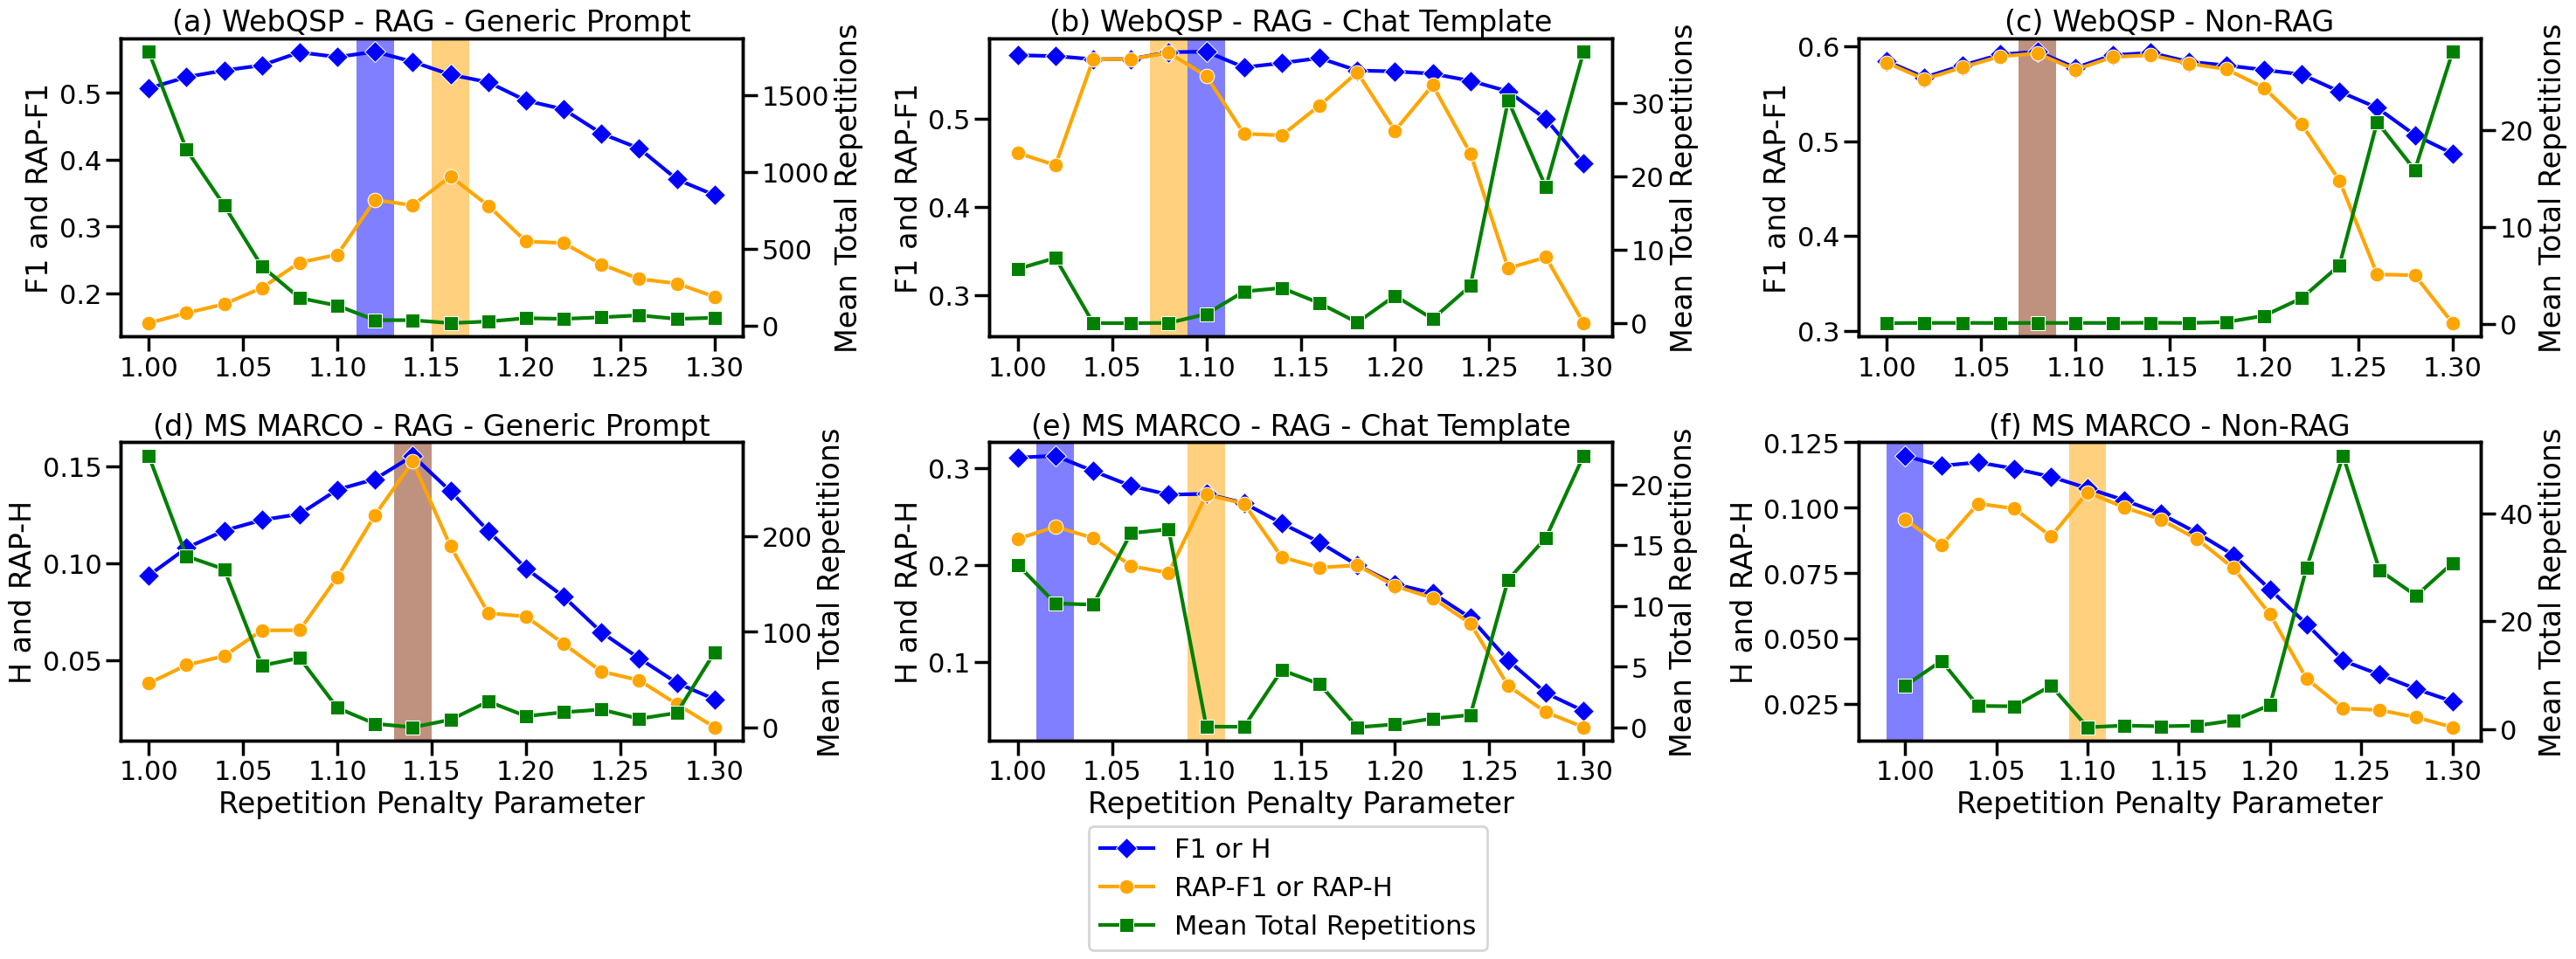
\includegraphics[width=\textwidth]{image/RPP Tuning.png}
% \caption[Performance vs. Repetition Trade-Off]{This figure illustrates the balance between performance and reducing excessive repetition for the Phi-3-mini model across various datasets and prompt types. The blue line is for F1, the orange line is for \mtr, and the green line indicates \rap. These visualizations help discern how a model’s performance and repetition behavior vary with different RPP values.}
%Performance vs. Repetition Trade-Off. This figure illustrates the balance between performance and reducing excessive repetition for the Phi-3-mini model across various datasets and prompt types. The blue lines represent the original performance (F1 or overall performance) scores, the orange lines (scaled on the right y-axis) denote the mean total repetitions (MTR) across the dataset, and the green lines indicate the repetition-aware performance (RAP), which is the original performance adjusted by $\log_{10}(10 + \alpha \times \text{MTR})$, with $\alpha$ fixed at 1 in this study. In these graphs, the blue vertical bar is centered around the RPP (Repetition Penalty Parameter) that yields the best original performance, while the orange bar is positioned at the RPP with the best RAP. In subplots (a), (b), (e), and (f), these two bars are distinctly separated, whereas in subplots (c) and (d), they overlap, resulting in a combined color (likely brown) due to the blending of blue and orange. These visualizations help discern how a model’s performance and repetition behavior vary with different RPP values, thereby aiding in determining the optimal prompts and RPP settings for any AI task.
% \label{fig:performance_vs_repetition}
% \end{figure*}



% \begin{figure*}[ht]
% \centering
% 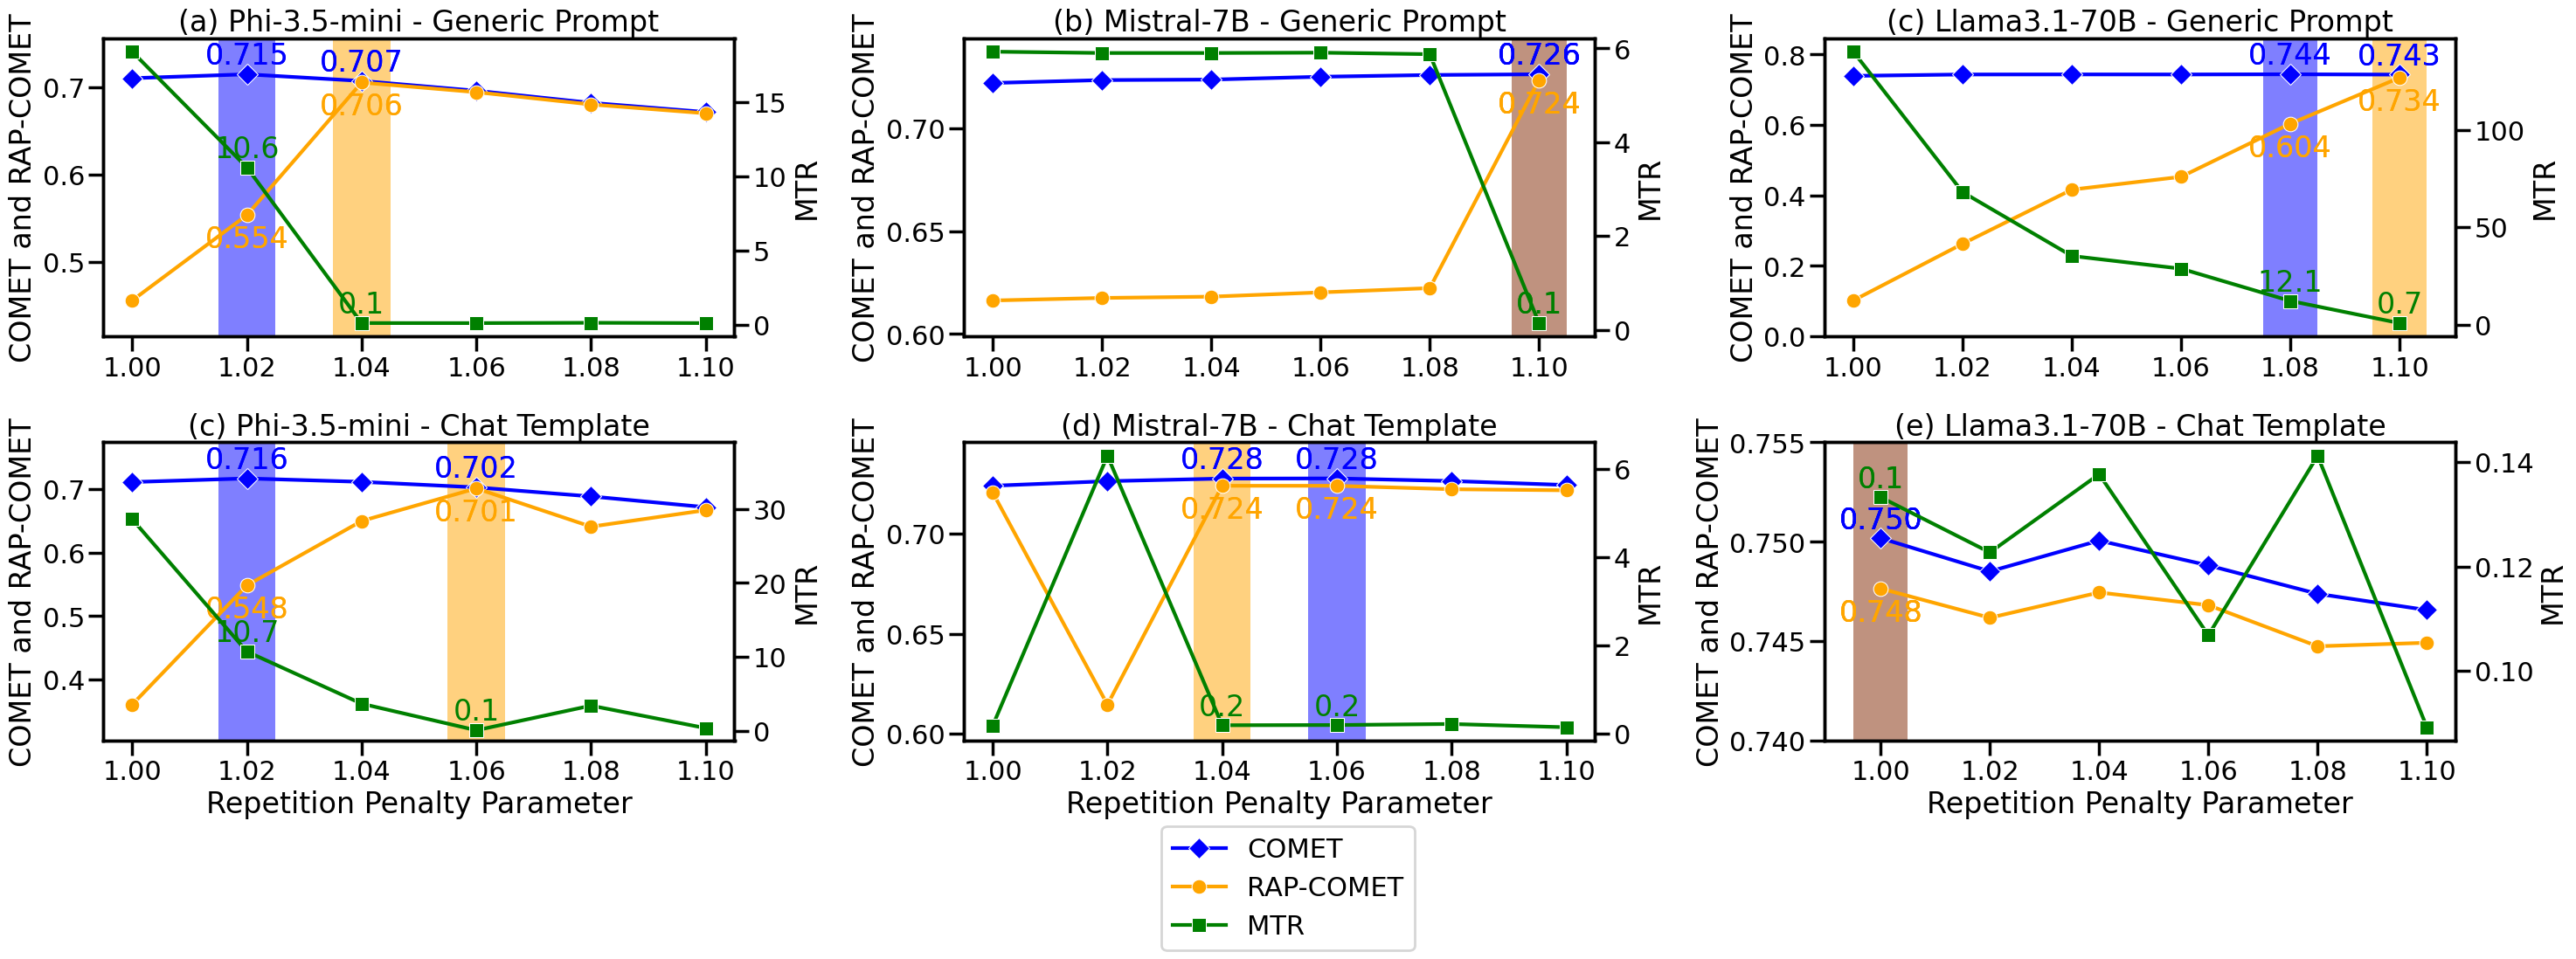
\includegraphics[width=\textwidth]{image/performance_vs_repetition_mt.png}
% \caption[Performance vs. Repetition Trade-Off for MT Tasks]{\new{Performance vs. Repetition Trade-Off for MT Tasks. This figure illustrates the trade-off between performance and the reduction of excessive repetition for the Phi-3.5-mini, Mistral-7B, and Llama3.1-70B models across both Generic Prompt and Chat Template prompt types. The blue line represents COMET, the orange line represents \mtr, and the green line represents \rap. The blue shaded region highlights the Repetition Penalty Parameter (RPP) for the best COMET performance, while the orange region highlights the RPP for the best RAP-COMET performance. When both bars overlap, the shaded region changes to brown to indicate this alignment.}}
% \label{fig:performance_vs_repetition_mt}
% \end{figure*}

% \subsection{Comparing the Best Repetition-Aware Performance of All the Models}
% \todo{@Donghao: to add table of best performance based on RAP. Maybe can use this section to compare the methods, use table. So this is to give people a sense of how the models perform, quantivatively}
% Performance Comparison based on Best \rap
% Comparing Performances of All Models selected based on best \rap. }
% Compare the Performance using tuned RPP (based on RAP)
% \input{tab_best_rpp_v2}
% \input{tab_best_rpp_v3}
% \input{tab_best_rpp_v4}

\subsection{Comparing the RAP-Tuned Performance of All Models}
Table \ref{tab:model-performance} shows the performance of the open-source LLMs after tuning \rpp using \rap. 
On \textbf{WebQSP}, Mistral-7B leads for both \raggen and \ragtem, scoring 0.609 and 0.604, respectively. However, Llama-3-70B outperforms all models in the \nonrag prompt with a high F1 score of 0.710. 
For \textbf{MS MARCO}, Gemma-1.1-2B excels in both \ragtem and \nonrag, with scores of 0.277 and 0.250, while Llama-3-70B takes the top spot in \raggen with 0.275.
In the MT task (\textbf{MAC}), Llama3.1-70B dominates both the generic prompt and chat template categories, scoring 0.743 and 0.750.
These results show that larger models like Llama-3-70B and Mistral-7B consistently achieve top performance across datasets and prompting strategies. However, mid-sized models like Gemma-1.1-2B perform competitively on specific tasks, such as MS MARCO, highlighting that model choice should be task-dependent and not solely based on model size.


% In this section, we analyze the RAP-tuned performance of various models on two different tasks: QA (Question Answering) and MT (Machine Translation). Table \ref{tab:model-performance} provides a comprehensive comparison of model performances across different datasets and prompt types. 
% For the QA task, on the \textbf{WebQSP} dataset, the \textbf{Mistral-7B} model achieves the highest performance for \raggen and \ragtem, with scores of 0.609 and 0.604, respectively. The best \nonrag performance is observed from \textbf{Llama-3-70B}, scoring an impressive 0.710.

% On the \textbf{MS MARCO} dataset, \textbf{Gemma-1.1-2B} achieves top performance for both \ragtem and \nonrag, with scores of 0.277 and 0.250, respectively. The best \raggen score for MS MARCO is achieved by \textbf{Llama-3-70B}, with a score of 0.275.

% For the MT task, \textbf{Llama3.1-70B} dominates, showing the highest performance for both \mtgen and \mttem, with scores of 0.743 and 0.750, respectively.

% These results demonstrate that larger models like \textbf{Llama-3-70B} and \textbf{Mistral-7B} consistently deliver top performance across various datasets and prompt types. However, mid-sized models such as \textbf{Gemma-1.1-2B} also perform competitively, especially on specific tasks like MS MARCO, suggesting that model selection should be guided by task-specific needs and performance trade-offs rather than size alone.




% Our proposed framework, \ours, enables tuning \rp to find the trade-off between repetition and performance, as shown in Section \ref{sec:eval_tuning}. Now, we compare the performances of all the open-source LLMs using the \rp, selected based on \rap. 
% Table \ref{tab:best_rpp} compares the performance of the open-source LLMs across two datasets, WebQSP and MS MARCO, using different prompting strategies: \raggen, \ragtem, and Non-RAG. 
% %
% For the WebQSP dataset, Mistral-7B achieves the best results with both \raggen and \ragtem strategies. In the Non-RAG category, Llama-3-70B excels. Notably, the best result for non-RAG prompting is higher than that in RAG. We argue that since we provide information retrieved from documents instead of a knowledge graph, it might not be sufficient to answer questions from KBQA task that would requires many relational information. This can be seen in the opposite observation in \ms dataset where both RAG prompting strategies obtain much higher scores than non-RAG. 
% The table also highlights the performance penalties due to repetition. For instance, Phi-3-mini using \raggen has an F1 score of 52.7, but its \rap drops to 37.5 due to repetition. A similar trend is observed with Gemma-1.1-7b under the \raggen strategy.
% We also present the best results tuned based on the original F1 scores for \webqsp (denoted as [MODEL-NAME]-F1). This is to demonstrate the potential impact of not considering repetition when tuning \rp. We observed that using our framework, \ours, significantly reduces the repetition issue, with minimal changes in overall performance. For instance, with Llama-2-7B \raggen, an \rp of 1.0 yields the best F1 score of 60.1 but has a high repetition rate of 78.48 on average. However, using \ours, we can select the \rp of 1.06 which drastically reduces the mean total repetition to 0.01, while still achieving a comparable F1 score of 58.9. Several other similar cases are highlighted in blue text, illustrating the effectiveness and benefits of our framework in balancing repetition and performance.
% \todo{to revise, remove framework, to use metric}
% Our proposed framework, \rap, allows tuning \rp to balance repetition and performance, as shown in Section \ref{sec:eval_tuning}. We compare the performances of all open-source LLMs using the selected \rp based on \rap.
% Table \ref{tab:best_rpp} shows the performance of these LLMs across WebQSP and MS MARCO datasets with different prompting strategies: \raggen, \ragtem, and Non-RAG. For WebQSP, Mistral-7B performs best with \raggen and \ragtem, while Llama-3-70B excels in Non-RAG. Interestingly, the best Non-RAG result is higher than RAG, likely because document retrieval may not provide sufficient relational information needed for KBQA tasks. This contrasts with the MS MARCO dataset, where both RAG strategies outperform Non-RAG.
% The table also shows the performance penalties due to repetition. For example, Phi-3-mini using \raggen has an F1 score of 52.7, but its \rap drops to 37.5 due to repetition, a trend also seen with Gemma-1.1-7b under \raggen.
% We also present the best results tuned based on original F1 scores for \webqsp, denoted as [MODEL-NAME]-F1, to show the impact of not considering repetition when tuning \rp. Using our metric, \rap, significantly reduces repetition with minimal performance changes. For instance, with Llama-2-7B \raggen, an \rp of 1.0 yields an F1 score of 60.1 but has a high repetition rate of 78.48. However, with \ours, an \rp of 1.06 reduces repetition to 0.01, still achieving an F1 score of 58.9. Other similar cases are highlighted in blue, demonstrating our framework’s effectiveness in balancing repetition and performance.

% For the MS MARCO dataset, the performance trends shift. The Llama-3-70B model stands out under the \raggen strategy, achieving the highest F1 (33.7) and RAP (33.7) scores. Gemma-2B and Mistral-7B perform best for the RAG-Chat Template and Non-RAG strategies, respectively. There are significant drops from RAG to non-RAG performances. This is due to the difficulty of \ms questions and the high quality of relevant data provided in RAG prompts for \ms. 
% Overall, for both WebQSP and MS MARCO, most models exhibit zero or very low repetition (MTR), demonstrating the effectiveness of \ours in choosing \rp for balancing repetition and performance.

